\section{先行研究}
こうしたSNNにおける時間的特性の課題に対して, 先行研究では時定数を学習可能とし, その多様性を実現することが多く行われている\cite{dhsnn, yin2020effective, paramsnn}.
本節では, ニューラルネットワークの重みとバイアスと同様に, 時定数を学習可能とした手法について述べる.
さらに, 1つのニューロンに対して複数の時定数を割り当てることで, SNNの時間的特性を向上させた手法について記述する.

\subsection{Parametric-SNN}
前述の通り, LIFモデルで構成されたSNNの学習アルゴリズムでは, 膜電位の時定数はハイパーパラメータとして扱われる.
そのため, SNNの学習ではニューロン間の接続重みとバイアスのみが最適化される.
しかし, 時系列入力に対するSNN内のニューロンダイナミクスは, その時定数による影響を無視できない.
ある単一のニューロンにおける入力と膜電位の関係の模式図を\figref{fig:lif}に示す.
ニューロンは膜電位$V$を持ち, その値は前方のニューロンからの入力$I$によって変化する.
さらに, その変化量は前方のニューロンの接続重み$w$とそのニューロンの時定数$\tau$に依存する.
また, ニューロンに定常入力が加わったときの膜電位の時間変化を\figref{fig:liffigure}に示す.
ここで, 曲線origin(青線)は時定数$\tau$と重み$w$が基準値のときの膜電位の時間変化を表す.
一方で, $w^+, \tau^+$はそれぞれ重みと時定数が基準値より大きい場合の膜電位の時間変化を表す.
また, $w^-, \tau^-$はそれぞれ重みと時定数が基準値より小さい場合の膜電位の時間変化を表す.
\figref{fig:liffigure}より, ニューロンの接続重み$w$だけでなく, 時定数$\tau$の値によっても膜電位の収束速度が変化することがわかる.
このことから, 時定数を学習可能とすることで, SNNの時間表現能力の向上が期待される.
\begin{figure}[htbp]
    \centering

    \parbox{1.0\textwidth}{
        \centering

        \begin{minipage}{0.243\textwidth}
            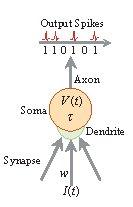
\includegraphics[width=1.0\textwidth]{Static/chap1_paramsnn_neuronmodel.pdf}
            \subcaption{LIFモデル}
            \label{fig:lif}
        \end{minipage}
        \hspace{0.02\textwidth}
        \begin{minipage}{0.657\textwidth}
            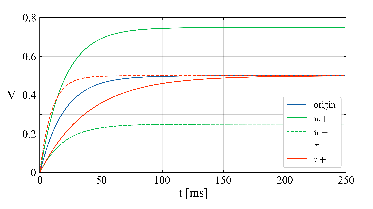
\includegraphics[width=1.0\textwidth]{Static/chap1_paramsnn_volttrj.pdf}
            \subcaption{LIFモデルにおける膜電位変化}
            \label{fig:liffigure}
        \end{minipage}

        \caption[LIFモデルの模式図と膜電位の時間変化]{
            \cite{paramsnn}
            (a) LIFニューロンモデルの模式図. $I, V$はそれぞれニューロンへの入力と膜電位. 
            $w, \tau$はそれぞれニューロン間の接続重みと時定数. 
            (b) ニューロンに定常入力が加わったときの膜電位の時間変化. 
            $+, -$はそれぞれのパラメータの大小を表す.
        }
    }
\end{figure}

Fangらは, このようなSNNの時定数を学習可能としたアルゴリズムとしてParametric-SNNを提案した\cite{paramsnn}.
Parametric-SNNでは, ニューロンの重み$w$と同様に時定数$\tau$が学習中に最適化される.
そのため, 事前に時定数をハイパーパラメータとして設定する必要がない.
また, SNNの同じ層ではニューロン間の時定数が共有される.
これは, 脳における隣接するニューロンは類似の時間特性を持つ特徴を反映しており, 生物的妥当性が高い.
一方, 異なる層間では時定数は共有されず, 異なる値を持つ.
これによって, SNNが多様な時間的特性の学習が可能となる.
結果として, Parametric-SNNは従来のLIFモデルを用いたSNNよりも画像認識, 動画認識タスクにおいて高いパフォーマンスを発揮した (\tabref{tab:paramsnn:result1}).
さらに, その学習の収束速度も向上することが示された (\figref{fig:paramsnn:traincurve}).
\begin{table}[htbp]
    \centering
    \caption[Parametric-SNNのパフォーマンス]{
        Parametric-SNNのパフォーマンス\cite{paramsnn}.
        タスクは画像認識, 動画認識のベンチマークテスト. 
        $\tau$は学習前の時定数の初期値を表す.
    }
    \label{tab:paramsnn:result1}
    {\small %12ptだとはみ出るので小さく
    \begin{tabular}{ccccc}
        \hline
        Model & Fashion-MNIST & CIFAR-10 & CIFAR10-DVS & DVS128 Gesture\\
        \hline
        Parametric-SNN ($\tau_0=2$) & \textbf{94.38 \%} & \textbf{93.50 \%} & \textbf{74.80 \%} & \textbf{97.57 \%}\\
        SNN ($\tau=2$) & 94.17 \% & 93.03 \% & 73.60 \% & 96.88 \%\\
        \hline
        Parametric-SNN ($\tau_0=16$) & \textbf{94.65 \%} & \textbf{93.23 \%} & \textbf{70.50 \%} & \textbf{92.01 \%}\\
        SNN ($\tau=16$) & 94.47 \% & 47.50\% & 62.40 \% & 76.74 \%\\
        \hline
    \end{tabular}
    }
\end{table}

\begin{figure}[t]
    \centering
    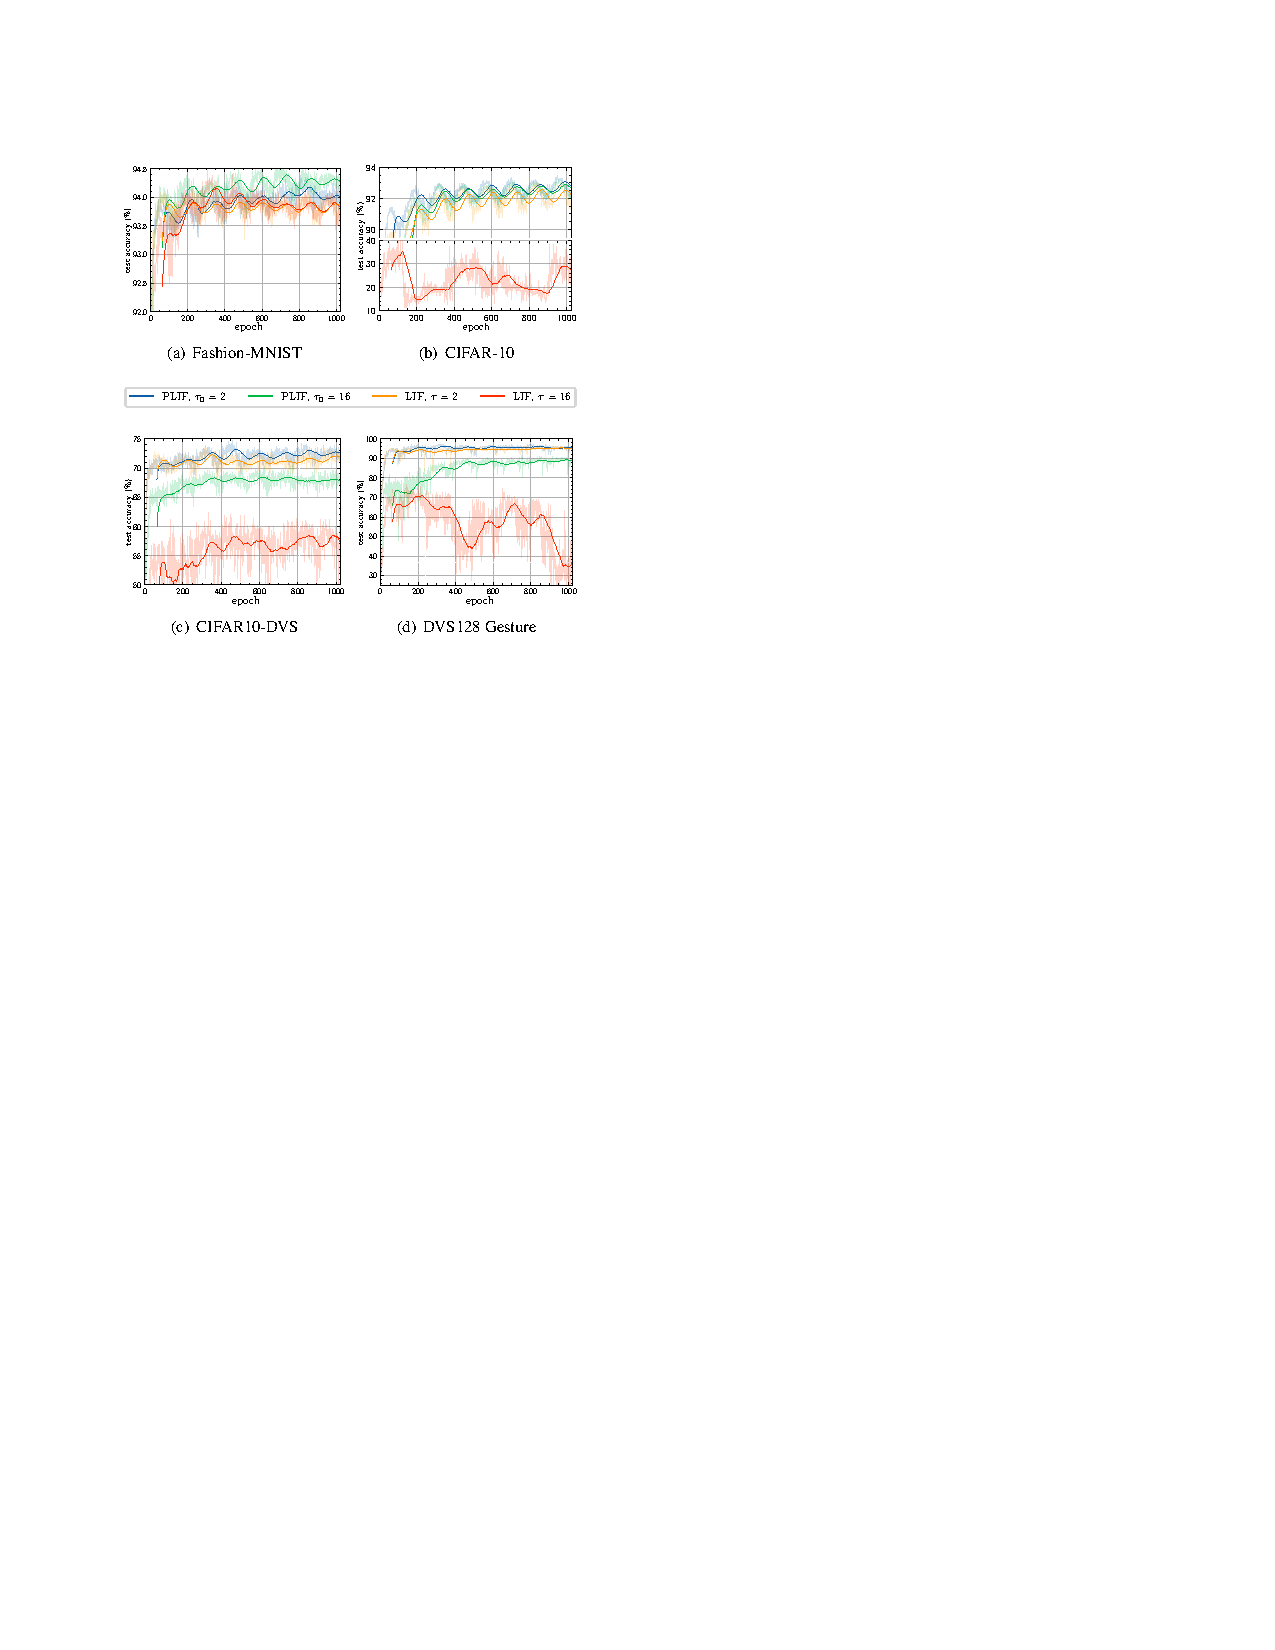
\includegraphics[width=0.8\textwidth]{Static/chap1_paramsnn_traincurve.pdf}
    \caption[Parametric-SNNとSNNの学習曲線]{
        Parametric-SNNとSNNの学習曲線\cite{paramsnn}.
    }
    \label{fig:paramsnn:traincurve}
\end{figure}


\subsection{DH-SNN}
Parametric-SNNでは, 時定数を学習可能とすることで, ニューロンダイナミクスの時間特性に対して多様性を与えた.
しかし, ニューロンへの入力に対する時間的特性については考慮されていない.
\figref{fig:single:neuron}に単一ニューロンの模式図を示す.
ニューロンの内部状態$u$は, ニューロンへの入力$i$によって変化する.
ここで, 入力$i$は前方に接続されたニューロンからの信号が直接伝達されるわけではない.
枝枯れした樹状突起と呼ばれる構成要素が前方のニューロンからの信号を受け取る.
その後, それぞれの樹状突起からの信号の総和がニューロンへの入力となる.
脳では, ニューロンの多様な時間的特性に加えて, それぞれの樹状突起も異なる時間的特性を持つことで, 複雑な時間表現を可能にしている.
しかしながら, LIFモデルや先行研究では, この樹状突起の時間特性の多様さは考慮されていない.
\begin{figure}
    \centering

    \parbox{1.0\textwidth}{
        \centering

        \begin{minipage}{0.42325\textwidth}
            \includesvg[width=1.0\textwidth, inkscapelatex=false]{Static/chap1_dhsnn1}
            \subcaption{単一ニューロン}
            \label{fig:single:neuron}
        \end{minipage}
        \hspace{0.02\textwidth}
        \begin{minipage}{0.477\textwidth}
            \includesvg[width=1.0\textwidth, inkscapelatex=false]{Static/chap1_dhsnn2}
            \subcaption{DH-SNNにおける単一ニューロンの概要図}
            \label{fig:dhsnn}
        \end{minipage}

        \caption[DH-SNNにおける単一ニューロンの模式図]{
            \cite{dhsnn}
            (a) 単一ニューロン. $i, u$はそれぞれニューロンへの入力と膜電位. 
            ニューロンへの入力$i$は, 枝分かれした樹状突起からの信号の総和としてモデル化される.
            (b) DH-SNNにおける単一ニューロンの概要図.
            $\alpha_i$はそれぞれの樹状突起の持つ時定数を表す.
            $\beta$はニューロンの持つ時定数を表す.
        }
    }

    % \vspace{0.5cm}

    % \parbox{1.0\textwidth}{
    %     \centering
    %     \includesvg[width=0.9\textwidth, inkscapelatex=false]{Static/chap1_dhsnn3}
    %     \label{fig:dhsnn:network}
    %     \caption[DH-SNNのネットワーク構造]{
    %         DH-SNNのネットワーク構造\cite{dhsnn}
    %     }
    % }
\end{figure}

Zhengらは, このような樹状突起の時間特性の多様さを表現するDH-SNNを提案した.
\figref{fig:dhsnn}にDH-SNNにおける単一ニューロンの概要図を示す.
時定数$\beta$を持つ1つのニューロンに対して, $d$個の樹状突起を接続する.
さらに, それぞれの樹状突起に対して$\alpha$で表される時定数を割り当てる.
このニューロンの時定数$\beta$と樹状突起の時定数$\alpha$を学習することで, より複雑な時間情報の学習が可能になる.
また, DH-SNNは長期の時間依存関係の学習にもその有効性が示された.
通常, ニューロンの膜電位はその活性によって電気パルス信号を出力すると, その状態は初期状態にリセットされる.
そのため, LIFモデルは長期の時間関係の記憶が困難とされている.
一方, 樹状突起ではそのリセットが生じないため, より長期の時間関係の学習が可能となる.
DH-SNNを用いることで, 音声認識や動画認識, 脳波認識において, 通常のSNNと比較して高いパフォーマンスを発揮した\figref{fig:dhsnn:voice}\figref{fig:dhsnn:brain}.
\begin{figure}
    \centering

    \parbox{1.0\textwidth}{
        \centering

        \begin{minipage}{0.5336\textwidth}
            \includesvg[width=1.0\textwidth, inkscapelatex=false]{Static/chap1_dhsnn4}
            \subcaption{音声認識}
            \label{fig:dhsnn:voice}
        \end{minipage}
        \hspace{0.02\textwidth}
        \begin{minipage}{0.3663\textwidth}
            \includesvg[width=1.0\textwidth, inkscapelatex=false]{Static/chap1_dhsnn5}
            \subcaption{脳波認識}
            \label{fig:dhsnn:brain}
        \end{minipage}

        \caption[DH-SNNにおける精度比較]{
            \cite{dhsnn}
            (a) 音声認識タスク精度比較.
            (b) 脳波認識タスク精度比較.
        }
    }
\end{figure}
